% !TEX TS-program = pdflatex
% !TeX encoding = UTF-8
% !TeX spellcheck = en_GB

\documentclass[aspectratio=43]{beamer}
% use this instead for 16:9 aspect ratio:
%\documentclass[aspectratio=169]{beamer}
% supported acpect ratios  1610  169 149 54 43 (deault) 32
%

\usepackage[english]{babel}
\usepackage[utf8]{inputenc}
\usepackage[T1]{fontenc}
\usepackage{amsmath}
\usepackage{algorithm}
\usepackage[noend]{algpseudocode}
\usepackage{appendixnumberbeamer}
\usepackage{tikz}
\usetikzlibrary{calc}

%% Create argmax and argmin operators.
%% Thin space, limits underneath in displays.
\DeclareMathOperator*{\argmin}{arg\,min}
%% Thin space, limits underneath in displays.
\DeclareMathOperator*{\argmax}{arg\,max}

\newcommand{\deq}{\dot{=}}
\newcommand{\tikzmark}[1]{\tikz[overlay,remember picture] \node (#1) {};}

\usetheme{ETHbeamer}

\colorlet{ETHcolor1}{ETHc}
\colorlet{ETHcolor2}{ETHc}

\author{Kevin Klein}

\title{Characterizing and Approximating the Optimal Allocation for Top-$m$ Arm
    Identification}

\date{2019-11-27}

% uncomment if you do not want to use a department logo
%\deplogofalse


\begin{document}

\titleframe

\begin{frame}
\frametitle{Context}
\begin{itemize}[<+->]
  \item Bandits, arms $[k]$.
  \item Reward distributions: 1-dimensional exponential family.
  \item Frequentist setting: true means $\theta^*$ and $m$ true best arms
      $S^* \subset [k]$.
  \item Top-$m$ arm identification goal: identifying $S^*$ with high confidence and few samples.
  \item Confidence: $\max_{S} \Pr[S \text{ is top-}m | \mathcal{D}_n]$ with $S \subset [k]$ and $|S| = m$.
  \item Fixed vs adaptive.
  \item Allocation $\psi$ with $\psi_{n, l} = \Pr[I_n = l]$.
\end{itemize}
\end{frame}

\begin{frame}
  \begin{figure}[h]
    \centering
    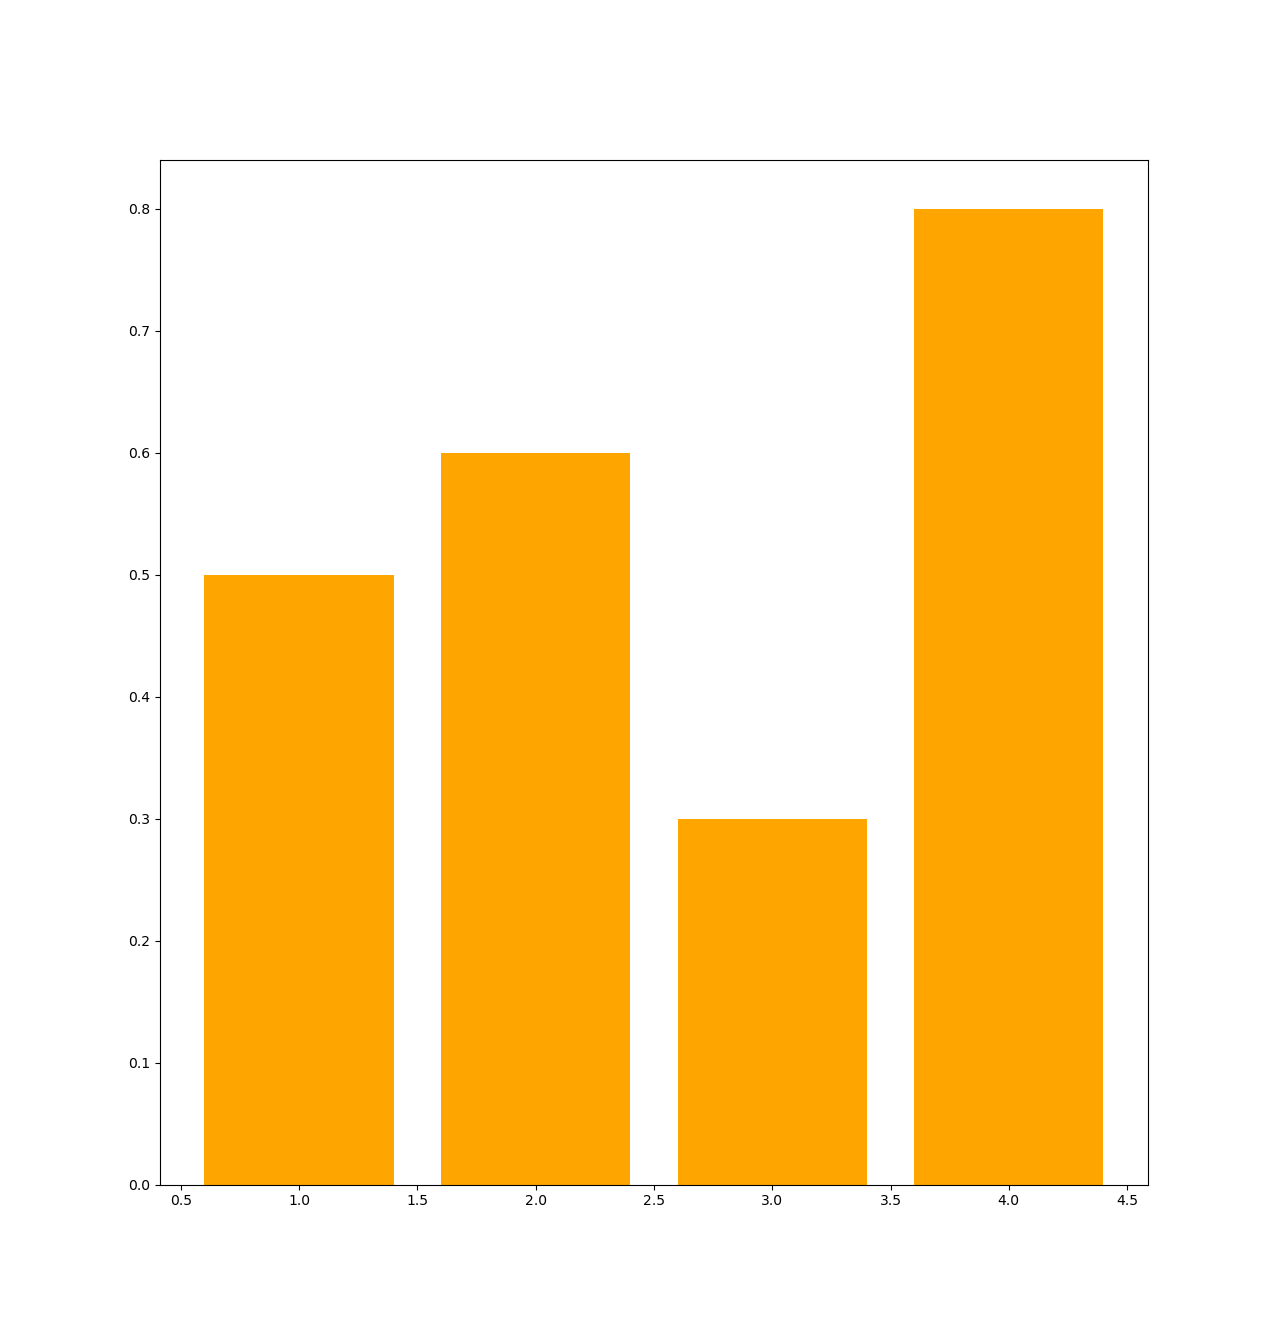
\includegraphics[width=.5\textwidth]{191127-bandits_1.png}
    \caption{Arms and their true means $\theta^*$. $k=4$.}
  \end{figure}
\end{frame}

\begin{frame}
  \begin{figure}[h]
    \centering
    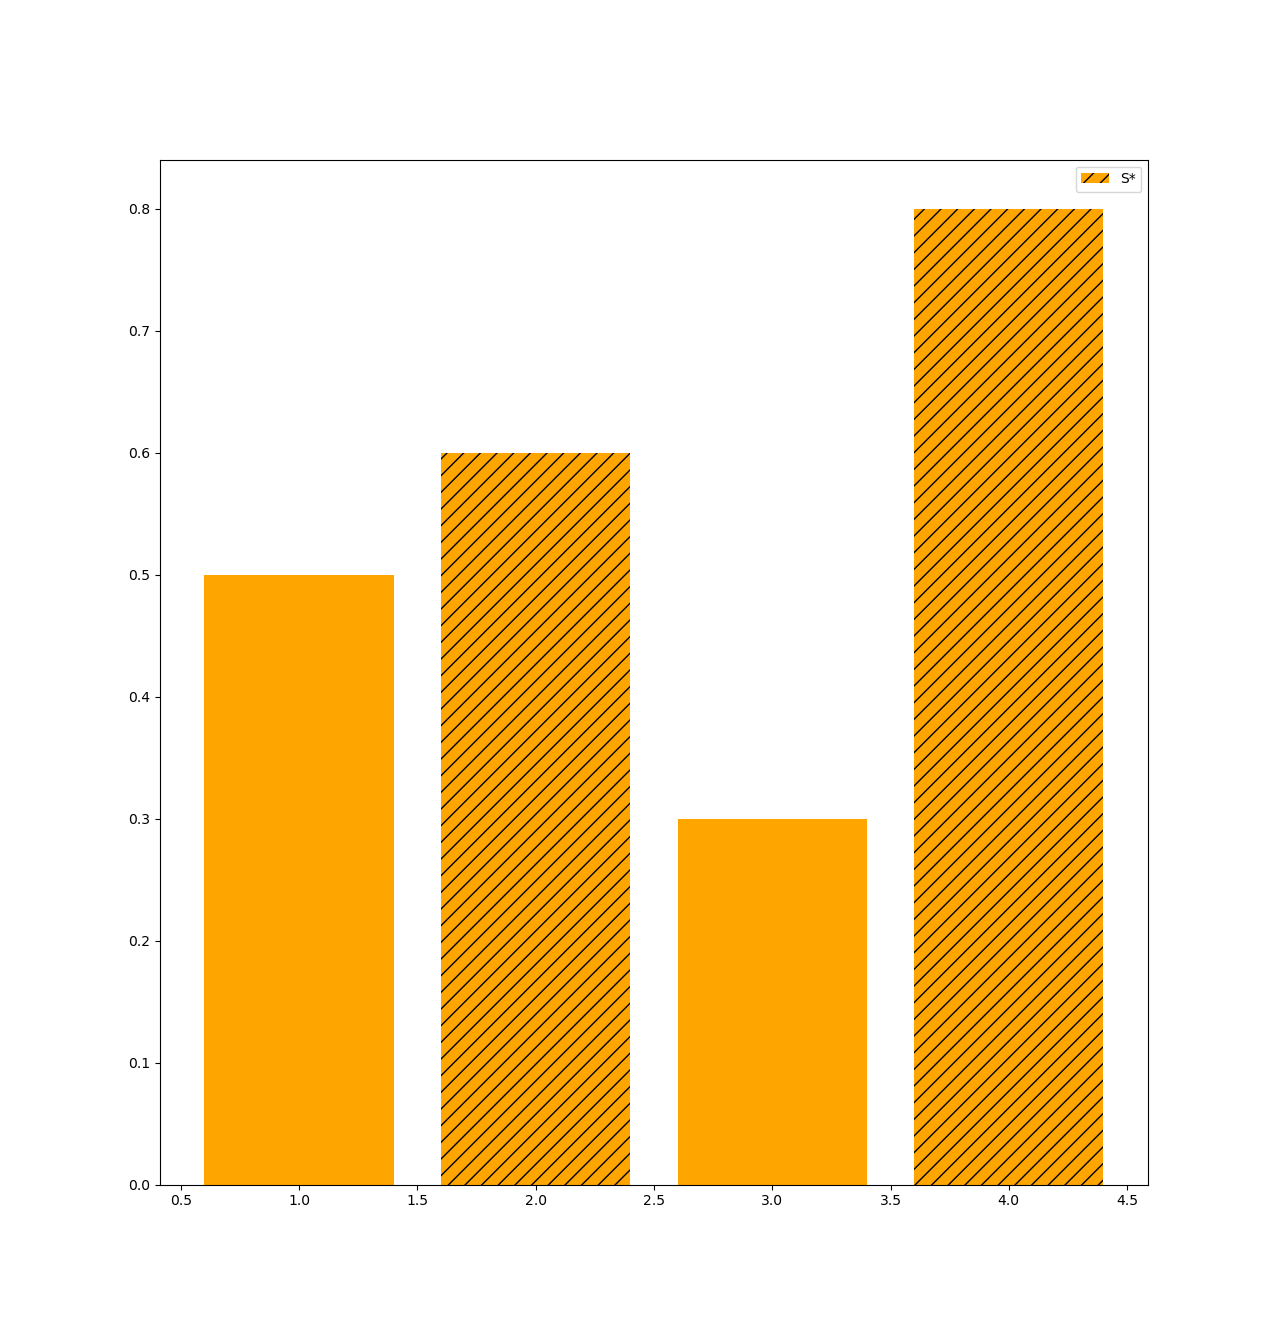
\includegraphics[width=.5\textwidth]{191127-bandits_2.png}
    \caption{Arms, their true means $\theta^*$ and $S^*$. $k=4$, $m=2$.}
  \end{figure}
\end{frame}

\begin{frame}
\frametitle{Credit}
Most of the work is inspired by Daniel Russo's \emph{Simple Bayesian
algorithm for Best Arm Identification} \footnote{\url{https://arxiv.org/
abs/1602.08448}}.
\end{frame}

\begin{frame}
\frametitle{Optimality of fixed allocation}
\begin{itemize}[<+->]
  \item $\Pr[S^* \text{ is top-}m | \mathcal{D}_n] \rightarrow 1$ with $n
      \rightarrow \infty$ is not hard.
  \item What's hard: converge optimally fast.
  \item Goal: Maximize rate at which $\Pr[S^* \text{ is top-}m |
      \mathcal{D}_n] \rightarrow 1$ with $n \rightarrow \infty$.
  \item We prove that for any fixed allocation $\psi$:
    \begin{align}
      &\Pr[S^* \text{ is top-}m | \mathcal{D}_n] \\
      &\approx 1 - \exp\{-n \min_{i \notin S^*} \min_{j \in S^*}
          \tikzmark{infrastructure}{\min_{x \in \mathbb{R}} \psi_i
          d_{KL}(\theta^*_i || x) + \psi_j d_{KL}(\theta^*_j || x)} \}
    \end{align}
  \item As a consequence, the optimal minimizes the exponent.
  \[\psi^* = \argmax_{\psi} \min_{i \notin S^*}\min_{j \in S^*} \min_{x \in
      \mathbb{R}} \psi_i d_{KL}(\theta^*_i || x) + \psi_j d_{KL}(\theta^*_j || x)\]
\end{itemize}
\pause\tikz[overlay,remember picture]{\draw[draw=red,thick,fill
    opacity=0.2] ($(infrastructure)+(-0,0.4)$) rectangle
    ($(infrastructure)+(4.9,-0.2)$);}
\end{frame}

\begin{frame}
\frametitle{Evidence for distinction}
\begin{itemize}[<+->]
  \item $C_{j, i}(\psi_j, \psi_i) = \min_{x \in \mathbb{R}} \psi_i d_{KL}
      (\theta^*_i || x) + \psi_j d_{KL}(\theta^*_j || x)$
  \item Distinction comprises both frequency $\psi$ and distance of values,
      captured by KL divergence.
\end{itemize}
\end{frame}

\begin{frame}
\frametitle{Characterization}
\ETHbox{\textwidth}{% define the ETHbox
\onslide<1->{
  \begin{theorem}[Characterization of optimal allocation]
  There is a unique fixed allocation $\psi^*$ maximizing the convergence rate of the posterior mass put on the true best arms. It enforces that:
  \[\forall j_1, j_2 \in S^*, \forall i_1, i_2 \notin S^*:
    C_{j, i}(\psi^*_{j_1}, \psi^*_{i_1}) = C_{j, i}(\psi^*_{j_2},
    \psi^*_{i_2})\]
  \end{theorem}}}
  \onslide<2->{
  This leads to a slightly simpler convergence rate for the optimal allocation:
  \[\Pr[S^* \text{ is top-}m |
      \mathcal{D}_n] \approx 1 - \exp\{-n\ C_{j, i}(\psi^*_j, \psi^*_i)\}\]
  for any $j \in S^*$, $i \notin S^*$.}
\end{frame}

\begin{frame}
\frametitle{Example: Setup}
\begin{itemize}[<+->]
  \item Top-4.
  \item Given true underlying means:
    \begin{align}
      \theta^1 &= [.1,\ .2,\ .3,\ .4,\ .5,\ \underbrace{.6,\ .7,\ .8,\
    .9}_\text{$S^*$}] \\
      \theta^2 &= [.4,\ .425,\ .45,\ .475,\ .5,\ \underbrace{.525,\ .55,\
    .575,\ .6}_\text{$S^*$}]
    \end{align}
  \item Overdetermined system of equations: Find $\psi$ such that $\forall j_1,
    j_2 \in S^*, \forall i_1, i_2 \notin S^*: C_{j, i}(\psi_{j_1}, \psi_{i_1})
    = C_{j, i}(\psi_{j_2}, \psi_{i_2})$.
\end{itemize}
\end{frame}

\begin{frame}
\frametitle{Example: Resulting allocation}
\begin{figure}[h]
  \centering
  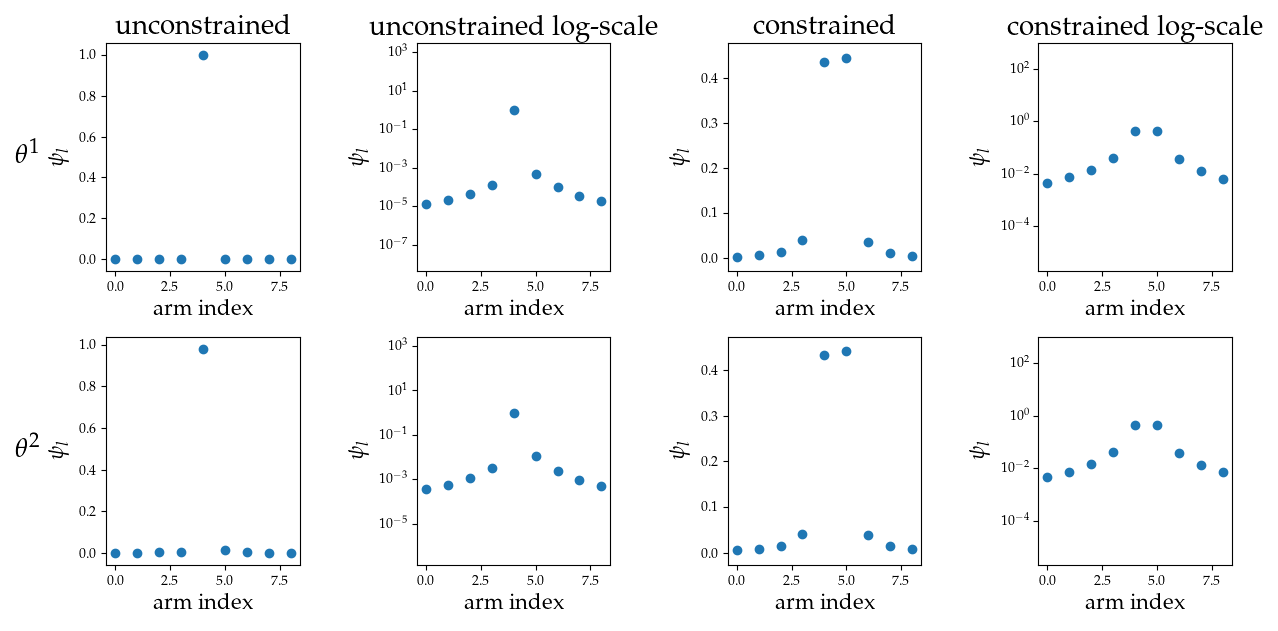
\includegraphics[width=\textwidth]{optimal_allocation.png}
  \caption{Unconstrained and constrained optimal allocation for $\theta^1$ and $\theta^2$, top-4.}
  \label{fig:optimal_allocation}
\end{figure}
\end{frame}

\begin{frame}
\frametitle{Top-2$m$ XOR Thompson sampling}
\begin{itemize}[<+->]
  \item Adaptive.
  \item Simple.
  \item Bayesian (remember: confidence).
  \item Asymptotic consistency.
  \item Based on Thompson sampling and another layer of randomization.
  \item Idea: Always sample two distinct candidates.
  \item Goal: Convergence towards optimal fixed allocation.
\end{itemize}
\end{frame}

\begin{frame}
\frametitle{TXTS: Algorithm}
\begin{algorithm}[H]
  \caption{TXTS: Given a posterior $\Pi_{n-1}$ in step $n$.}
  \label{alg:TXTS}
  \begin{algorithmic}
    \State $\hat{\theta} \sim \Pi_{n-1}$
    \State $S_1 =$ top-$m(\hat{\theta})$
    \Repeat
      \State $\hat{\theta} \sim \Pi_{n-1}$
      \State $S_2 = $ top-$m(\hat{\theta})$
    \Until{$S_1 \neq S_2$}
    \State $I_n \sim \mathcal{U}(S_1 \oplus S_2)$
    \State Play $I_n$, observe reward and update posterior.
  \end{algorithmic}
\end{algorithm}
\end{frame}

\begin{frame}
  \frametitle{TXTS: Exemplary candidates}
  \begin{figure}[h]
    \centering
    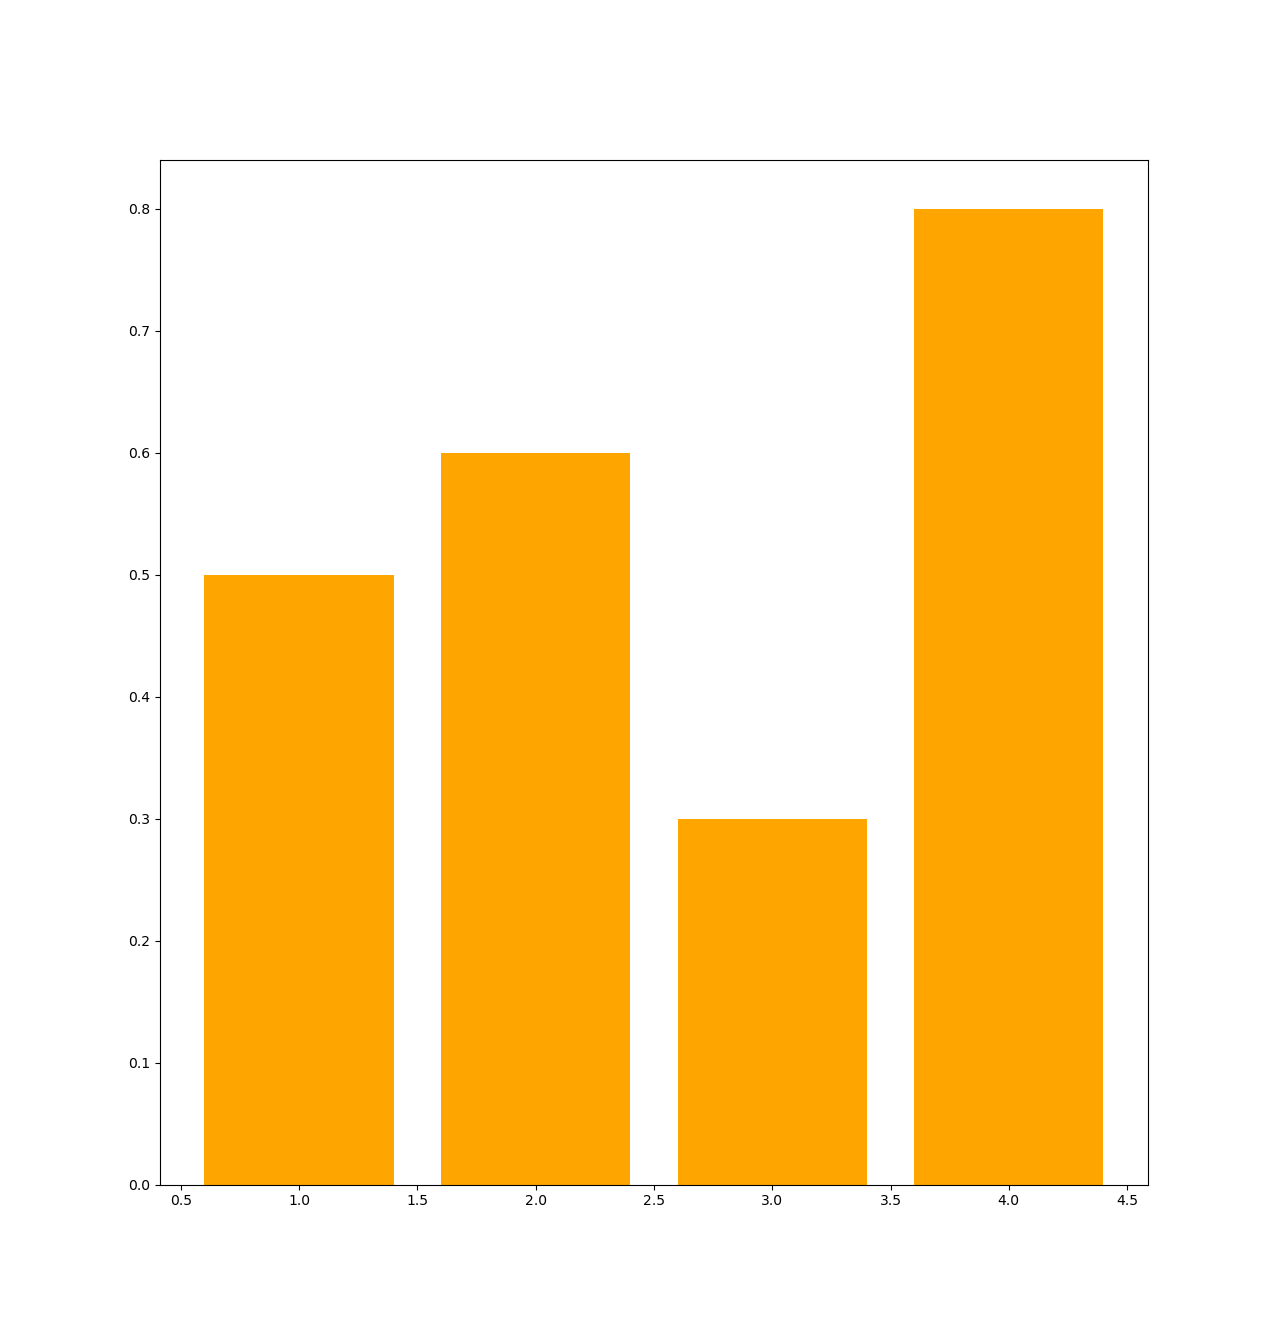
\includegraphics[width=.5\textwidth]{191127-bandits_1.png}
    \caption{Arms and their true means $\theta^*$. $k=4$.}
  \end{figure}
\end{frame}

\begin{frame}
  \frametitle{TXTS: Exemplary candidates}
  \begin{figure}[h]
    \centering
    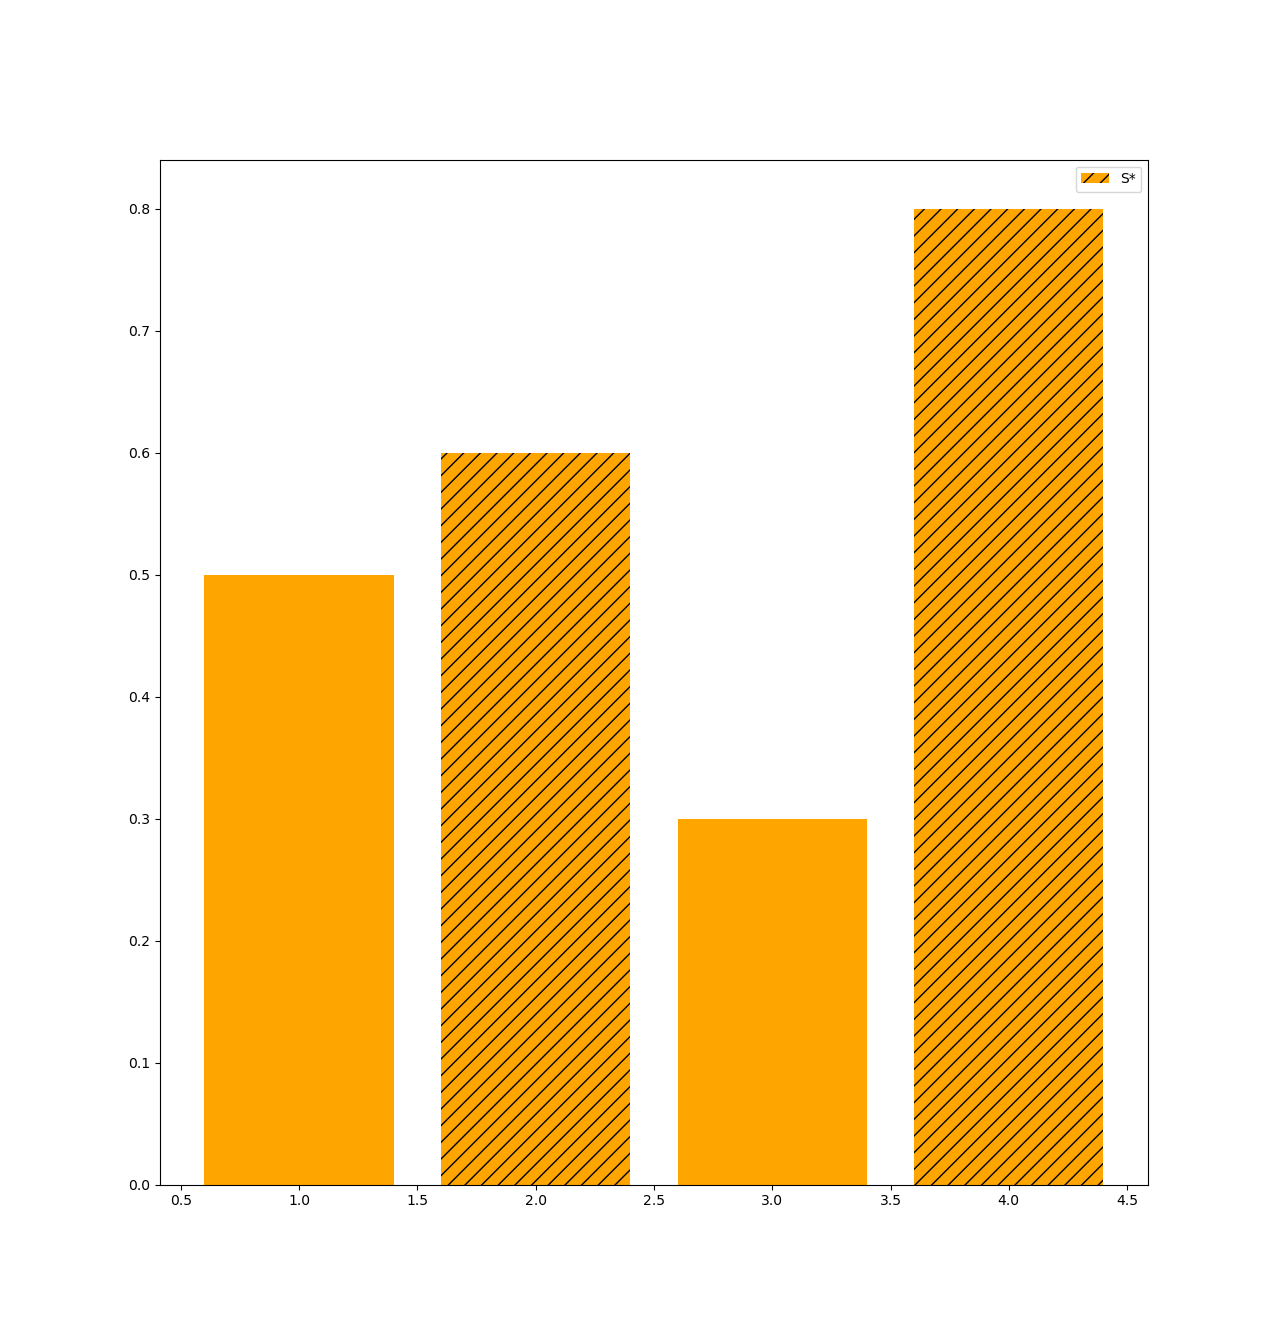
\includegraphics[width=.5\textwidth]{191127-bandits_2.png}
    \caption{Arms, their true means $\theta^*$ and $S_1$. $k=4$, $m=2$.}
  \end{figure}
\end{frame}

\begin{frame}
  \frametitle{TXTS: Exemplary candidates}
  \begin{figure}[h]
    \centering
    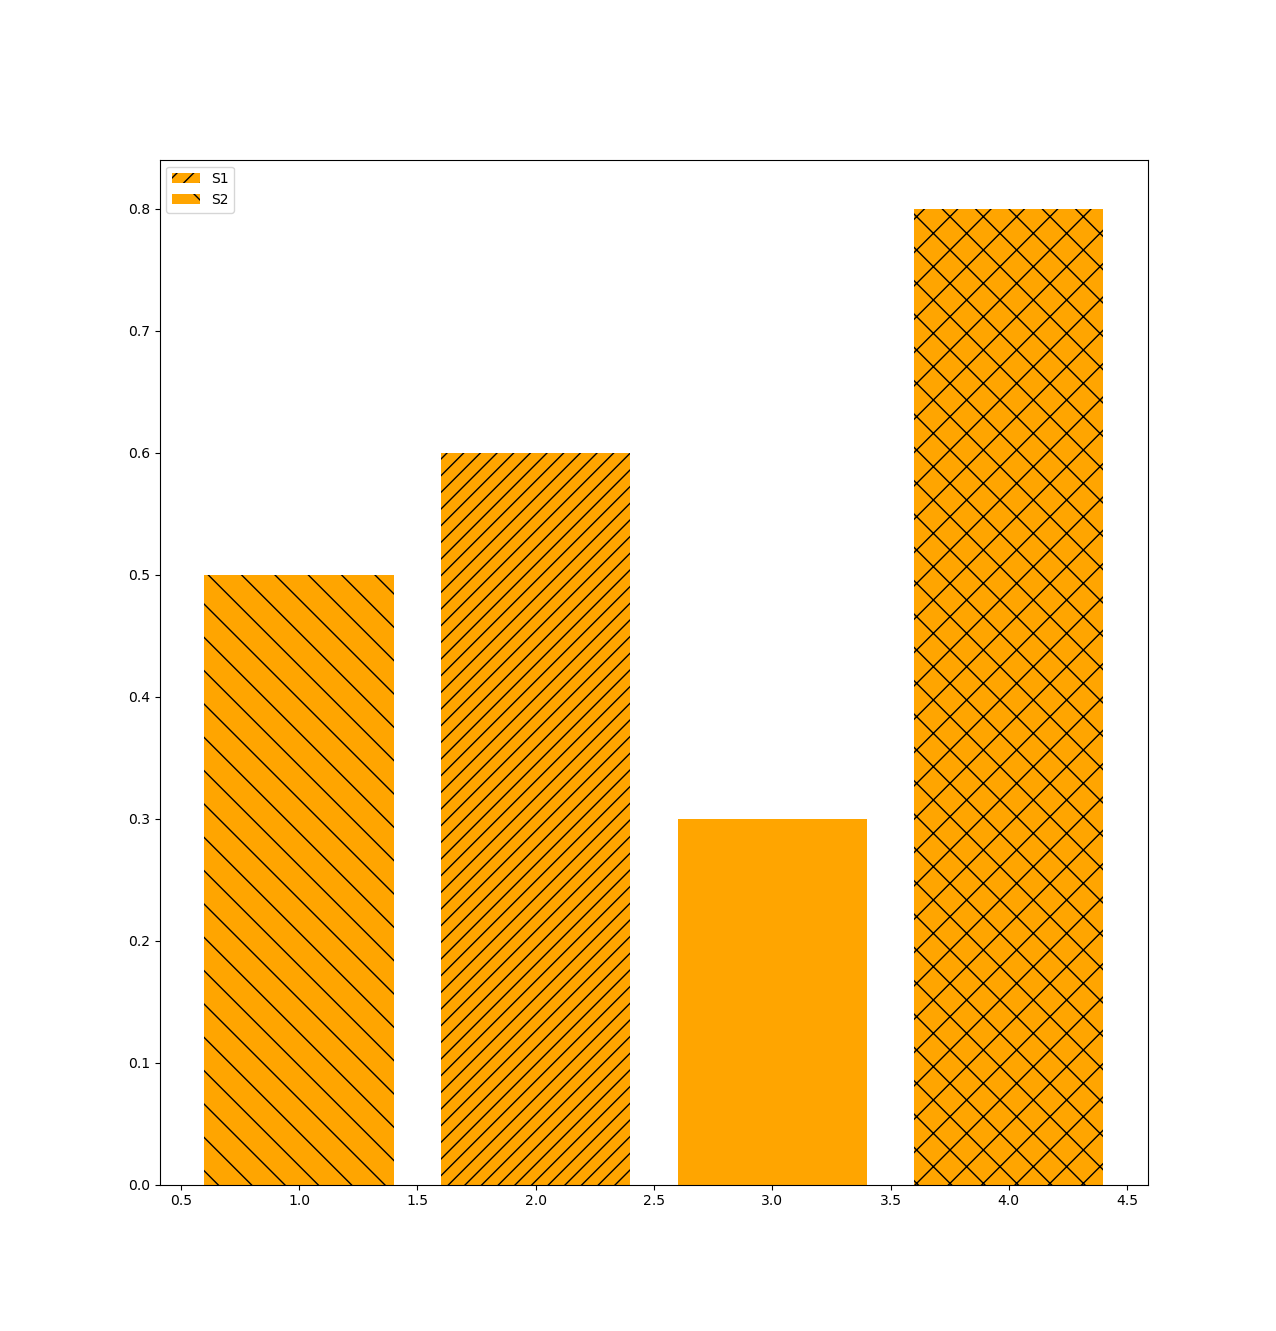
\includegraphics[width=.5\textwidth]{191127-txts_2.png}
    \caption{Arms, their true means $\theta^*$, $S_1$ and $S_2$. $k=4$, $m=2$.}
  \end{figure}
\end{frame}

\begin{frame}
\frametitle{TXTS: Empirical results}
\begin{itemize}[<+->]
  \item Bernoulli rewards.
  \item Beta posteriors, $\alpha = \beta = 1$.
  \item Top-4.
  \item $\theta^* = [.1,\ .2,\ .3,\ .4,\ .5,\ \underbrace{.6,\ .7,\ .8,\
          .9}_\text{$S^*$}]$
\end{itemize}
\end{frame}

\begin{frame}
\frametitle{TXTS: Evidence collection}
\begin{figure}[h]
  \centering
  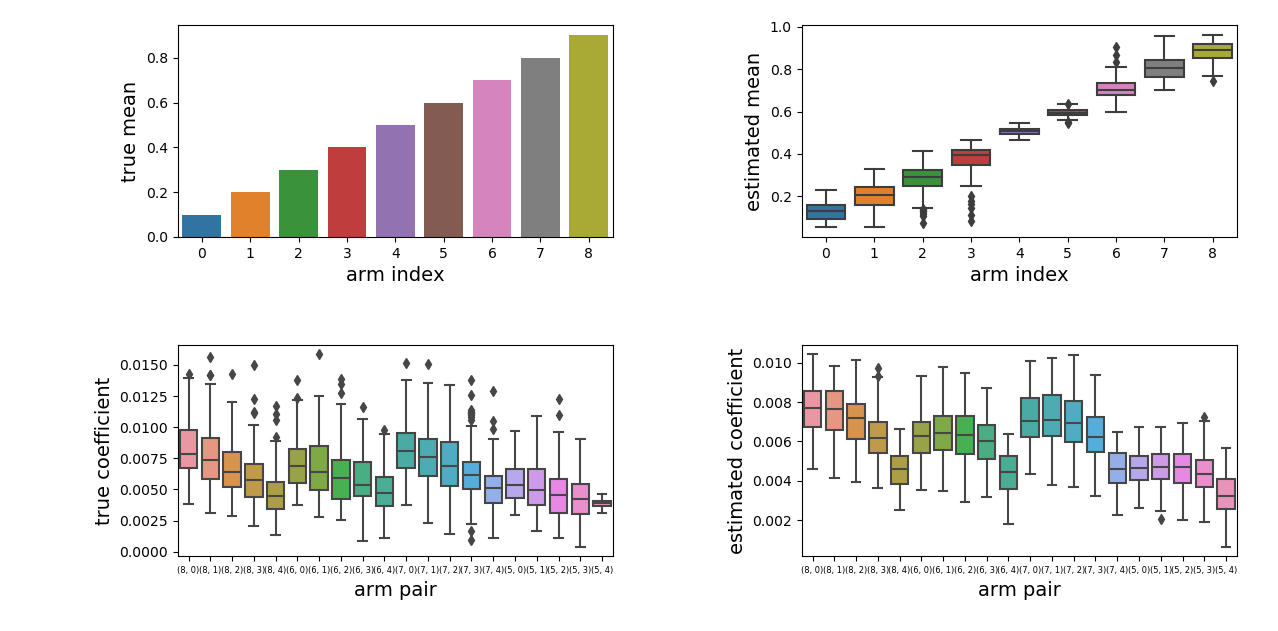
\includegraphics[width=\textwidth]{190909-coefficients_2000.png}
  \caption{Top row: true and estimated $\theta$. Bottom row: true and estimated
      coefficients $C_{j, i}$. 2000 steps, 150 seeds.}
  \label{fig:algorithm_coefficients}
\end{figure}
\end{frame}

\begin{frame}
\frametitle{TXTS: Empricial average allocation comparison}
\begin{figure}[h]
  \centering
  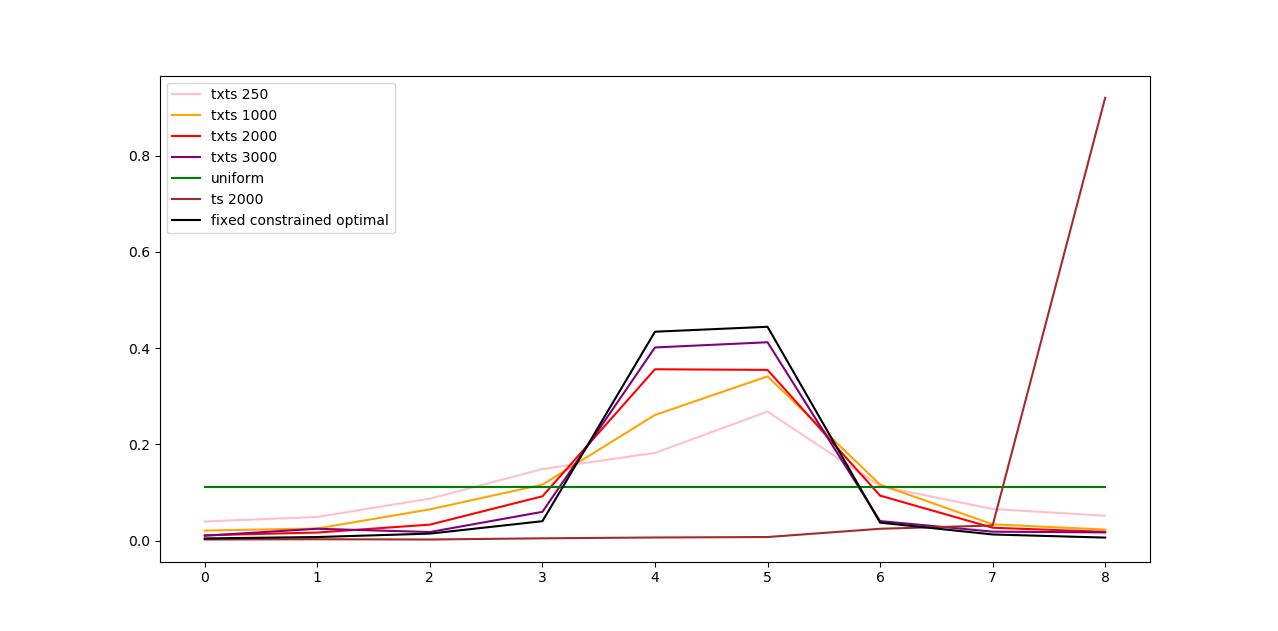
\includegraphics[width=\textwidth]{191127-allocations.png}
  \caption{Comparison of allocations for different methods and numbers of
      samples. 50 seeds.}
\end{figure}
\end{frame}

\begin{frame}
\frametitle{TXTS: Theoretical status quo}
\begin{itemize}[<+->]
  \item Allocation $\psi$ hard to explicitly express in closed form.
  \item Established bounds on $\psi$.
  \item Proven $\Pr[S^* \text{ is top-}m | \mathcal{D}_n] \rightarrow 1$.
  \item Proven $\sum_{j \in S^*} \psi_{n, S^*} \rightarrow \frac{1}{2}$.
  \item Proven that if converged on $S^*$, then convergence on $S^{*c}$ and
      vice versa.
  \item Proven some more technical statements.
\end{itemize}
\end{frame}

\begin{frame}
\frametitle{TXTS: Theoretical outlook}
Prove overall convergence, i.e. $\frac{1}{N}\sum_{n \in [N]} \psi_n \rightarrow \psi^*$.
\end{frame}

\begin{frame}
Thanks!
\end{frame}

\appendix

\begin{frame}
Appendix.
\end{frame}

\begin{frame}
\frametitle{1-d exponential family}
\begin{itemize}
  \item They have a scalar parameter $\theta$.
  \item They come with the definition of functions $T(x)$, $\nu(\theta)$, $h(x)$ and $A(\theta)$. $T$ corresponds to the sufficient statistic and $A$ to the log-partition function.
  \item The probability density function is defined by:
    \[f_X(x|\theta) = h(x) \exp(\nu(\theta) T(x) - A(\theta))\]
  \item They have conjugate priors.
  \item Bernoulli, binomial with known number of trials, Poisson,
      exponential, Pareto with known minimal value, chi-squared, normal
      distribution with known variance and more.
\end{itemize}
\end{frame}

\begin{frame}
\frametitle{Logarithmic equivalence}
Convergence is reasoned about in a $\deq$ sense, with:
\begin{align}
  a_n \deq b_n \Leftrightarrow \lim_{n \rightarrow
  \infty}\frac{1}{n}\log{\frac{a_n}{b_n}} \rightarrow 0
\end{align}
\end{frame}

\begin{frame}
\frametitle{Computing evidence}
The Bernoulli assumption allows us to solve the minimization over $x$ analytically.
\begin{align}
  d(\theta_l||x) &= \theta_l \log(\frac{\theta_l}{x}) + (1-\theta_l) \log(\frac{1-\theta_l}{1-x}) \label{eq:bernoulli_kl} \\
  x_0 &= \frac{\psi_j\theta_j + \psi_i\theta_i}{\psi_j + \psi_i}
\end{align}
\end{frame}

\begin{frame}
\frametitle{TXTS: Increase in confidence}
\begin{figure}[h]
  \centering
  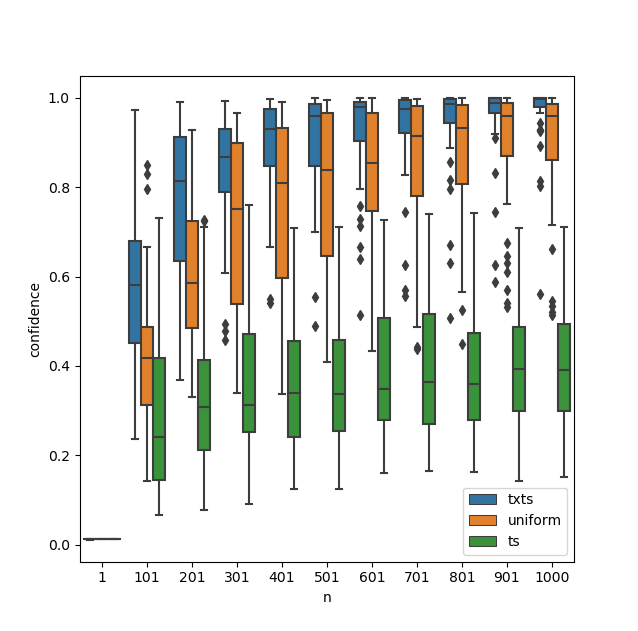
\includegraphics[width=.55\textwidth]{190723-confidences.png}
  \caption{Confidence per steps for TXTS, uniform and Thompson sampling. 50
      seeds.}
\end{figure}
\end{frame}

\begin{frame}
\frametitle{TXTS: Empirical average allocation}
\begin{figure}[h]
  \centering
  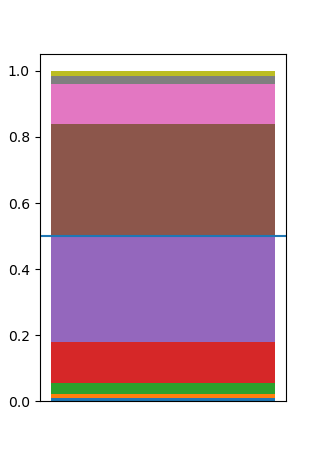
\includegraphics[width=.35\textwidth]{190723-selections_2.png}
  \caption{TXTS empirical average allocation after 1000 steps. Arms ordered by true mean. 50 seeds.}
\end{figure}
\end{frame}

\begin{frame}
\ETHbox{\textwidth}{
  \begin{theorem}[Sufficient condition for optimality]
    If
    \begin{align}
      \forall l \in [k], \delta > 0: \sum_{n \in \mathbb{N}} \psi_{n, l}
          \mathbb{I}[\bar{\psi}_{n, l} \geq \psi^*_l + \delta] < \infty
    \end{align}
    then $\bar{\psi}_{n} \rightarrow \psi^*$.
  \end{theorem}
}
\end{frame}
\end{document}
